\documentclass[12pt]{article}
\usepackage[T1]{fontenc}
%\usepackage[latin9]{inputenc}
\usepackage[utf8]{inputenc}
\usepackage[english]{babel}
\usepackage{amsmath}
\usepackage{amsfonts}
\usepackage{amssymb}
%\usepackage{setspace}
\usepackage{rotating}
\usepackage{graphics}
\usepackage{eurosym}
\usepackage[round]{natbib}
%\usepackage{graphicx}
%\usepackage{float} 				%allows you to float images
\usepackage{latexsym}
%\usepackage{bbding}
%\usepackage {moresize}
\usepackage{listings}
\usepackage{bbding}
\usepackage{blindtext}
\usepackage{hhline}
\usepackage{tikz}
\usetikzlibrary{trees}
%\usetikzlibrary{shapes,backgrounds}
%\usepackage{pgfplots}
%\usetikzlibrary{arrows}
\usepackage{enumitem}
%\doublespacing
%\usepackage{geometry}
\usepackage{amsthm}
\usepackage{color}
%\usepackage{array,multirow}
%\usepackage{subcaption}
%\usepackage{pst-plot}
%	\psset{xunit=15mm}
%\geometry{verbose,tmargin=1in,bmargin=1in,lmargin=.5in,rmargin=.5in}
\setlength{\parskip}{\bigskipamount}
\setlength{\parindent}{0pt}
\usepackage{multicol}

\newenvironment{problem}[3][Problem]{\begin{trivlist}
\item[\hskip \labelsep {\bfseries #1}\hskip \labelsep {\bfseries #2.}]}{\end{trivlist}}

\newcommand{\barr}{\bar{r}}
\newcommand{\ddx}{\frac{d}{dx}}
\newcommand{\infsum}{\sum_{n=1}^{\infty }}

\title{Problem Set 4 \thanks{Problems:5.2,5.4,5.6,5.7,5.12,5.16,5.17,5.20,5.27}}
\author{Ian McGroarty \\
	Course Number: 555.444}
\date{September 23, 2019}

\begin{document}

\maketitle
\newpage
%%%%%%%%%%%%%%%%%%%%%%%%%%%%%%%%%%%%%%%%%%%%%%%%%%%%%%%%
%%%%%%%%%%%%%%%%%%%%%%%%%%%%%%%%%%%%%%%%%%%%%%%%%%%%%%%%
%%%%%%%%%%%%%%%%%%%%%%%%%%%%%%%%%%%%%%%%%%%%%%%%%%%%%%%%
\begin{problem}{5.2}. Wat is the difference between the forward price and the value of a forward contract?  \\
	\textbf{Def: Forward Price} The delivery price in a forward contract that causes the contract to be worth zero. (pg. 8)\\
	\textbf{Def: Forward Contract} An agreement to buy of sell an asset at a certain future time for a certain price. (pg. 6). \\
Based on the definitions above it can be explained that the \underline{value} of the forward at time zero is 0, since the the delivery price is set equal to the forward price. However, since the delivery price is fixed and the forward price subject to change. Thus, the value of the forward contract will be how much an investor gains from holding the future a given time and is equal to the present value discounted difference between  forward price and delivery price. 
\end{problem}

\begin{problem}{5.4}. A stock index currently stands at 350. The risk-free interest is 8\% per annum with continuous compounding and the dividend yeild on the index is 4\% per annum. What should the forward price for a four month contract be? Well we have $S_0=350, r=0.08, t= 0.33$ and using equation (4.3 pg. 83) we can show that the continuous compounding yield is 0.03922. Thus: 
\begin{align*}
F_0 &= S_0e^{(r-q)T} && \text{Eqn. 5.3 pg. 115} \\
&= 350e^{(0.08-0.03922)0.333} \\
F_0 &= 354.7418
\end{align*}
\end{problem} 



\begin{problem}{5.6}. Explain carefully the meaning of the terms convenience yield and cost of carry. What is their relationship between futures price, spot price, convenience yield, and cost of carry? \\
\textbf{Def: Convenience Yield:} A measure of benefits form ownership of an asset that are not obtained by the holder of a long future contract on the asset. (pg. 126) \\
\textbf{Def: Cost of Carry:} The storage costs plus the cost of financing an asset minus the income earned on the asset. (pg. 126) \\
To explore the difference between these two concepts we must first place our mindset on consumption commodities, goods that have utility outside of the investment realm such as milk \#buttercreamcapital. The convenience yield of milk after you just ate a big PB\&J skyrockets because there is a huge benefit of a nice cold glass of milk. Now assuming all the other wall street players also have PP\&J for lunch, that means that the cost of holding the milk futures is going to be lower. It is worth noting here that there is no financial or economic model that can accurately measure the sweet relief that comes with some chocolate milk (though it can be inferred if all other costs are known). But milk spoils... not to mention you have to keep it cold which means it takes up refrigerator space, and thus limits the amount of Coca-Cole the investment firm can keep. This would be reflected in the cost of carry. Clearly that would make it more costly to keep the milk pushing up the forward price.  
\end{problem}


\begin{problem}{5.7}. Explain why a foreign currency can be treated as an asset providing a known yield. \\
To understand why this is the case, we must first understand what is a known yield. Similar to a known income, a known yield is a perfectly predictable income (as a percentage of the held position) to the trader. In this way it is analogous to a risk free yield. Holding the currency in foreign dollars and receiving a risk free return in this country`s currency is thus the same as having a risk free yield in this country`s currency. So when calculating the value of holding in one currency versus another we must consider the difference of the two risk free yields. 
\end{problem}

\begin{problem}{5.12}. Risk Free interest rate is 10\% per annum (continuous compounding), and the dividend yield is 4\%. The index is standing at 400, and the futures price for a contract deliverable in 4 months is 405. What arbitrage opportunities does this create? \\
First, we use equation 5.3 (pg 115), $F_0 = S_0e^{(r-q)T}$ to see that the forward price is, $F_0 = 408.1039$. Clearly the actual price is too low relative to the theoretical price. What this means is we can short the index for \$405. Invest the money at the risk free rate, $405\cdot e^{0.1*0.33} = \$418.588 $. Or else, we can enter into futures contracts and hold on to them, and then sell in 4 months as the futures will have converged to the true value.
\end{problem}

\begin{problem}{5.16}. Prove that $F_2 \leq F_1e^{r(t_2-t_1)}$ no storage costs and r is constant.\\
Well suppose to the contrary that $F_2 > F_1e^{r(t_2-t_1)}$. Well then we could:
\begin{itemize}
\item Take a long position in $F_1$ (expiring at $t_1$) 
\item Take a short position in $F_2$. 
\item At $t_1$ borrow \$$F_1$ to repay long position (to be repaid at $t_2$). 
\item Then purchase \$$F_1$ of the asset 
\item At $t_2$ use the \$$F_1$ of the asset to make good on the short position of $F_2$.
\end{itemize}
This means you are paid $F_2$ and you borrowed: $F_1e^{r(t_2-t_1)}$. Since $F_2>F_1e^{r(t_2-t_1)}$ you`ve made a risk less profit! This can not be therefore our initial assumption must be incorrect. 
\end{problem} 

\begin{problem}{5.17}. The daily settlement process could lead to imperfect hedges if interest is applied to the margin account. \\
\textbf{a.} If  the value of the foreign currency falls rapidly during the life of the contract the investor will have to add money to the holder`s margin account. Meaning that they will miss out on the earned interest during that period. Whereas if they used a forward contract they would only pay the loss at the end. \\
\textbf{b.} If the foreign currency rises rapidly then the investor is better off since they will earn interest on the margin account which will be of greater value. \\
\textbf{c.} If the value of the currency first rises, the margin account will increase in value and the investor can earn interest on that money. Then the value falls back to the initial value its fine because the investor will still make money on the interest so they would still do better than the forward contract. \\
\textbf{d.} The interest on the margin account would be lower in this case meaning that they would stand to do better by investing in the forward contract. 
\end{problem}

\begin{problem}{5.20} Show that equation (5.3) is true: Explain what an arbitrager could do if 5.3 was not true. 
\begin{proof}
Equation 5.3 (pg. 115) states that $F_0 = S_0\cdot e^(r-q)T$ where $F_0$ is the forward price, $S_0$ is the current asset price, r is the risk free rate, q is the average yield per annum on an asset during the life of the contract, and  T is the tie of the contract. To see why this holds, consider the case where an investor buys one unit of the asset for $S_0$ and short sells the asset to be sold at $F_0$. This costs $S_0$ and will lead to a cash inflow of $F_0e^{qT}$ with present value $F_0e^{qT}e^{-rT}=F_0e^{(q-r)T}=S_0$ Or equivalently, $F_0 = S_0e^{(r-q)T}$. 
\end{proof}
If it were the case the $F_0 > S_0e^{(r-q)T}$ the future value is over priced. We can exploit that buy borrowing \$$S_0$ at the risk free rate in order to fund the purchase of one unit of the asset at \$$S_0$. Also at time zero we enter into a forward contract to lock in the sale of one unit of the asset at price $F_0$. When time T comes to pass, we owe $S_0e^rt$ and the value of the asset we own is $F_0e^{qt}$, but we can use the asset to cover the sale of the forward contract at the price $F_0$. So our net inflow/outflow is $F_0e^{qT}-S_0e^{rT}>0 \implies S_0e^{(r-q)T} < F_0$ 
If it were the case that $F_0 < S_0e^{(r-q)T}$. Then the future value is under priced. So we want to hold money and take advantage of the risk free rate. To get money now we short sell the asset for $S_0$ and immediately invest that money at the risk free rate. In order to cover our short position we need to enter into a forward contract to lock in a purchase at $F_0$ at time T. Then when time T comes, we enjoy the risk free inflow, use the the forward to cover the asset short, and by paying $F_0e^{qT}$. Thus, the net inflow/outflow is $S_0e^{rT} - F_0e^{qt} >0 \implies S_0e^{(r-q)T})>F_0$
\end{problem}

\begin{problem}{5.27}.  An index is 1200. The 3month r= 3\% and q=1.2\%. the 6 month r=3.5\% and q = 1\%. Estimate the futures price of the index for three month and 6 month contracts.\\
This is a straightforward application of equation 5.3 (pg 115). For the 3 month 
$$T=3/12=0.25 \implies F_0 = S_0e^{(r-q)T} = 1200\cdot e^{(0.03-0.012)\cdot 0.25} = 1205.412 $$
For the 6 month:
$$ T= 6/12 = 0.5 \implies F_0 = S_0e^{(r-q)T} = 1200\cdot e^{(0.035-0.01)\cdot 0.5} = 1215.094$$


\end{problem}


\end{document}



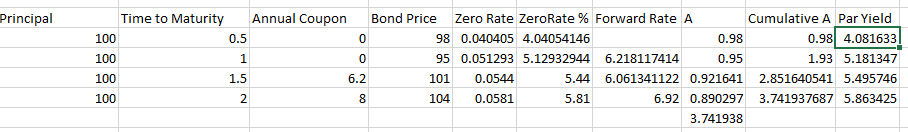
\includegraphics[width=\textwidth]{mod3_p434.png}
% Set the overall layout of the tree




\tikzstyle{level 1}=[level distance=3.5cm, sibling distance=3.5cm]
\tikzstyle{level 2}=[level distance=3.5cm, sibling distance=2cm]

% Define styles for bags and leafs
\tikzstyle{bag} = [text width=4em, text centered]
\tikzstyle{end} = [circle, minimum width=3pt,fill, inner sep=0pt]

\begin{tikzpicture}[grow=right, sloped]
\node[bag] {Bag 1 $4W, 3B$}
    child {
        node[bag] {Bag 2 $4W, 5B$}        
            child {
                node[end, label=right:
                    {$P(W_1\cap W_2)=\frac{4}{7}\cdot\frac{4}{9}$}] {}
                edge from parent
                node[above] {$W$}
                node[below]  {$\frac{4}{9}$}
            }
            child {
                node[end, label=right:
                    {$P(W_1\cap B_2)=\frac{4}{7}\cdot\frac{5}{9}$}] {}
                edge from parent
                node[above] {$B$}
                node[below]  {$\frac{5}{9}$}
            }
            edge from parent 
            node[above] {$W$}
            node[below]  {$\frac{4}{7}$}
    }
    child {
        node[bag] {Bag 2 $3W, 6B$}        
        child {
                node[end, label=right:
                    {$P(B_1\cap W_2)=\frac{3}{7}\cdot\frac{3}{9}$}] {}
                edge from parent
                node[above] {$B$}
                node[below]  {$\frac{3}{9}$}
            }
            child {
                node[end, label=right:
                    {$P(B_1\cap B_2)=\frac{3}{7}\cdot\frac{6}{9}$}] {}
                edge from parent
                node[above] {$W$}
                node[below]  {$\frac{6}{9}$}
            }
        edge from parent         
            node[above] {$B$}
            node[below]  {$\frac{3}{7}$}
    };
\end{tikzpicture}


\section{Definitions}
\underline{Def: Forward Rate Formulas} (pg 79). The implied forward rate between times $t_1$ and $t_2$ is the rate of interset between those times that is consistent with a given spot rate curve. For Yearly compounding, the forward rate is:  
\begin{align*}
f_{i,j} =& [\frac{(1+s_j)^j}{(1+s_i)^i}]^{1/(j-i)}-1 \\
 e^{s(t_2)t_2} =& e^{s(t_1)t_1}e^{f_{t_1,t_2}(t_2-t_1)}
\end{align*}

\underline{Discount Factor Relation} The discount facot between periods i and j is defined as $$ d_{i,j}=[\frac{1}{1+f_{i,j}}]^{j-i}$$ These factors satisfy the compounding rule: $d_{i,k}=d_{i,j}d_{j,k}$\\

\underline{Def. Derivative (Ross pg 223)} Let F be a real valued function defined on an open interval contained a point a. We say f is differentiable at a, or f has derivative at a if the limit $$ f'(a) = \lim_{x \to a} \frac{f(x)-f(a)}{x-a} $$




https://www.investopedia.com/university/advancedbond/bond-pricing.asp
https://quant.stackexchange.com/questions/22288/duration-of-perpetual-bond
http://people.stern.nyu.edu/gyang/foundations/sample-final-solutions.html
http://pages.stern.nyu.edu/~jcarpen0/courses/b403333/07convexh.pdf
https://web.stanford.edu/class/msande247s/2009/summer%2009%20week%205/Bond%20Formula%20Sheet.pdf


\underline{Def: Forward Rate Formulas} (pg 79). The implied forward rate between times $t_1$ and $t_2$ is the rate of interset between those times that is consistent with a given spot rate curve. For Yearly compounding, the forward rate is:  
\begin{align*}
f_{i,j} =& [\frac{(1+s_j)^j}{(1+s_i)^i}]^{1/(j-i)}-1 \\
 e^{s(t_2)t_2} =& e^{s(t_1)t_1}e^{f_{t_1,t_2}(t_2-t_1)}
\end{align*}

\underline{Discount Factor Relation} The discount facot between periods i and j is defined as $$ d_{i,j}=[\frac{1}{1+f_{i,j}}]^{j-i}$$ These factors satisfy the compounding rule: $d_{i,k}=d_{i,j}d_{j,k}$\\

\underline{Def. Derivative (Ross pg 223)} Let F be a real valued function defined on an open interval contained a point a. We say f is differentiable at a, or f has derivative at a if the limit $$ f'(a) = \lim_{x \to a} \frac{f(x)-f(a)}{x-a} $$



\begin{align*}
\text{Maximize  } & 4x_1 +5x_2 +3x_3 +4.3x_4 + x_5 + 1.5x_6 + 2.5x_7 + 0.3x_8 + x_9 + 2x_{10} \\
\text{Subject to } & 2x_1 + 3x_2 + 1.5x_3 + 2.2x_4 +0.5x_5 +15x_6 + 2.5x_7 +0.1x_8 + 0.6x_9 + x_{10} \leq 5 \\ 
& x_1 + x_2 + x_3 + x_4 \leq 1 \\
& x_5 + x_6 + x_7 \leq 1 \\
& x_8 + x_9 + x_{10} \leq 1 \\
\end{align*}